\documentclass[british,titlepage]{ntnuthesis}

\title{Long-term vessel trajectory inference using Gaussian Processes }
\shorttitle{Gaussian Process Trajectory Inference}
\author{%
Håvard Skåra Mellbye
\vspace{1cm}\\
Supervisor: Edmund Førland Brekke \\ 
Co-supervisor: Trym Tengesdal
}
\shortauthor{Mellbye}
\date{}


\addbibresource{thesis.bib}

\usepackage{tikz}
\usetikzlibrary{bayesnet}
\usepackage{ifthen}


% From https://www.overleaf.com/learn/latex/Glossaries

\makeglossaries % Prepare for adding glossary entries



% --------------------
% ----- Acronyms -----
% --------------------

\newacronym{mcmc}{MCMC}{Markov Chain Monte Carlo}
\newacronym{pgm}{PGM}{Probabilistic Graphical Model}
\newacronym{bp}{BP}{Belief Propagation}
\newacronym{dgm}{DGM}{Directed Graphical Models}
\newacronym{mrf}{MRF}{Markov Random Fields}
\newacronym{kl}{KL}{Kullback-Liebler divergence}
\newacronym{pdf}{PDF}{Probability Density Function}
\newacronym{pmf}{PMF}{Probability Mass Function}
\newacronym{vi}{VI}{Variational Inference}
\newacronym{elbo}{ELBO}{Evidence Lower Bound}
\newacronym{hmc}{HMC}{Hamiltonian Monte Carlo}

\newglossaryentry{moralization}
{
    name=moralization,
    description={The process of converting Directed Graphical Models into Markov Random Fields}
}

\newglossaryentry{support}{
    name=support,
    description={The set of possible outcomes/values with a non-zero probability, i.e. all events that can happen. A Gaussian distribution for example have support for $x \in \mathcal{R}$ since it has a non-zero probability, $p(x) > 0$, for all real numbers $x \in \mathcal{R}$.}
} % add glossary and acronym lists before document

\begin{document}

\chapter*{Abstract}

Autonomous ships depend on situational awareness in order to avoid collisions in a safe and robust manner. By knowing the intention of surrounding vessels, safety margins can be improved by avoiding situations with increased risk. In this thesis, methods for Bayesian Inference will be explored, with the goal of developing a flexible framework for intention modelling. Exact and approximate inference methods are explored. Approximate methods are found to be more flexible, allowing easier incorporation of existing knowledge from domain experts or conventions such as \Gls{colregs}. Methods such as \acrfull{mcmc} and \acrfull{vi} are therefore explored further and compared on an illustrative intention model. The results then find \acrshort{mcmc} to be accurate at the cost of computational complexity. \acrshort{vi} on the other hand, is found to be a lot faster, though much less precise on the illustrative model. 

\tableofcontents
\listoffigures
\listoftables
%\lstlistoflistings


\printglossary[type=\acronymtype] % Print acronyms
\printglossary                    % Print glossary

\chapter{Introduction}

\begin{figure}[h]
    \centering
    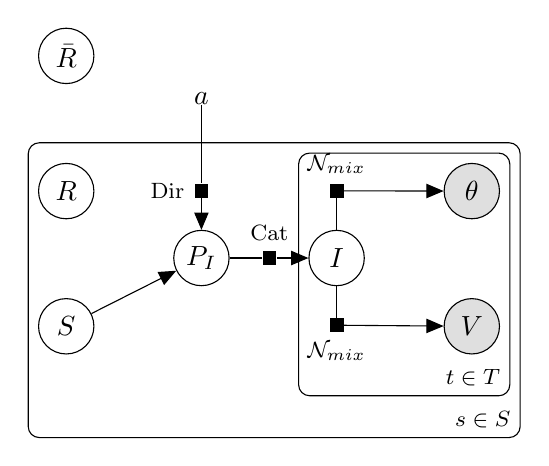
\begin{tikzpicture}
        % NODES
        \node[latent] (I) {$I$};
        \node[obs, right=of I, yshift=0.85cm] (theta) {$\theta$};
        \node[latent, left=of I] (PI){$P_I$};
        \node[obs, below=of theta] (V) {$V$};
        \node[latent, left=of PI, yshift=0.85cm] (R) {$R$};
        \node[latent, above=of R] (RR) {$\bar{R}$};
        \node[latent, below= of R] (S) {$S$};
        
        % FACTORS
        \factor[above=of I] {theta-f}{$\mathcal{N}_{mix}$}{}{};
        \factor[below=of I]{v-f}{below:$\mathcal{N}_{mix}$}{}{};
        \factor[left=of I]{I-f}{Cat}{}{};
        \factor[above=of PI]{PI-f}{left:Dir}{}{};

        \node[const, above=of PI-f] (a) {$a$};
        
        \factoredge {I} {theta-f} {theta};
        \factoredge {I} {v-f} {V};
        \factoredge{PI}{I-f}{I};
        \factoredge{a}{PI-f}{PI};

        \edge{S}{PI};

        \plate {ship}{(I)(theta)(V)}{$t \in T$};
        \plate {}{(I)(theta)(V)(R)(S)(ship)}{$s \in S$};
        
        
    \end{tikzpicture}
\end{figure}

\chapter{Neccessary Theoretical Background}

\section{Useful Results From Probability Theory}


 
\subsection{Conditional Probabilities}
The conditional probability $p(A | B)$ is the probability of $A$ occurring, given that we know $B$ has occured. 
\begin{equation}
    p(A | B) = \frac{p(A, B)}{p(B)}
\end{equation}



\section{Bayesian Statistics}

\section{Stochastic Modelling}

\section{Probabilistic Graphical Models}

\section{Belief Propagation}

\section{Markov Chains}


\chapter{Non-parametric trajectories using Gaussian Process}\label{chap:impl}
Predicting vessel trajectories can be parametrized in multiple ways. The simplest parametrization would be to directly model the trajectory $f(t)$ from observed data. Another approach is to rather learn a vector-field from AIS gradients, and use the vector field as variable input to a linear model. The vector-field can then be though of as forces, or flows, pushing the vessel in the direction of historical AIS data. A simple Kalman-filter predict step can then be used to simulate the movement for any vessel placed in the vector-field. 


\section{Non-parametric dynamic system using AIS tracking data}
The trajectory $\mathcal{T}$ can be expressed using the dynamical system
\begin{subequations}
\begin{align}
    \dot{\boldsymbol{x}} &= \vec{f}(\boldsymbol{x})\\
    \mathcal{T} &= \boldsymbol{x} + \epsilon, \quad \epsilon \sim \mathcal{N}(0, \sigma^2)
\end{align}
\end{subequations}

The function $\vec{f}(\cdot): \mathcal{R}^2 \to \mathcal{R}^2$ denotes the vector field describing the forces acting on a vessel. Normally this function is parametrized explicitly and the solution is solved either analytically or numerically depending on the complexity of the model. However, in the case of long-term prediction, the dynamics $\vec{f}(\cdot)$ is unknown and is unlikely stationary. Instead, the goal of this chapter is to use a \acrshort{gp} to create a non-parametric representation of the dynamics $\vec{f}(\cdot)$ by learning from historical trajectories of other vessels.

\begin{equation}\label{eq:gp_vec_field}
    \vec{f}(\boldsymbol{x}) = \begin{bmatrix} f_x (\boldsymbol{x})\\ f_y (\boldsymbol{x})\end{bmatrix} \sim \text{GP} \big(\begin{bmatrix} m_x(\boldsymbol{x})\\m_y(\boldsymbol{x})\end{bmatrix}, \ \begin{bmatrix}
    K_{xx}(\boldsymbol{x}, \boldsymbol{x}') & K_{xy}(\boldsymbol{x}, \boldsymbol{x}') \\ K_{xy}(\boldsymbol{x}, \boldsymbol{x}')^\intercal & K_{yy}(\boldsymbol{x}, \boldsymbol{x}')
    \end{bmatrix}\big) 
\end{equation}

The benefits of this formulation include:
\begin{description}
    \item[Easy incorporation of existing data] The model can easily be trained on partial data. Only the gradients of any historical trajectories are really needed.
    \item[Few constraining assumptions] The dynamical model is not constrained by any specific parametrization, while still allows prior knowledge such as smoothness to be incorporated into the model.
    \item[Uncertainty] The model can express uncertain when the availability of examples are sparse. 
\end{description}

The major downside is however that the model only learns gradients from data and relies heavily on numerical estimates of the velocity. In the case of AIS data, this is a large cause of uncertainty due to the large sampling interval.

The model could further be improved by clustering the samples based on similar behaviour for different ships, such as similarities in velocity. Separate \acrshort{GP}s could then be trained on the different subsets of data.

\cite{heinonen2018learningode} use a similar formulation to infer arbitrary, non-linear ODE models from sparse data and predict the dynamics far into the future. 



\section{Learning trajectories directly from data}
A more direct approach is to use a \acrshort{gp} to model a function $f: \mathcal{R}^5 \to \mathcal{R}^2$, mapping a ships current position $\boldsymbol{p}_t$, \acrshort{cog} $\psi_t$ and \acrshort{sog} $v_t$ to a position at time $t+\tau$. The method is formulated in mathematical terms in \cref{eq:gp_direct}. The model can then be queried about likely future positions by evaluating $\boldsymbol{f}$ with the desired initial conditions and time horizon, and then condition the \acrshort{gp} on close trajectories. 
The method simply boils down to using the \acrshort{gp} kernels to find trajectories with similar initial conditions, and use those to predict future positions.

\begin{subequations}\label{eq:gp_direct}
\begin{align}
    \boldsymbol{f}(\boldsymbol{x}) &= \boldsymbol{p}_{t+\tau} \label{eq:gp_direct_f}, \quad \boldsymbol{x} = \begin{bmatrix} \boldsymbol{p}_t & \psi_t & v_t & \tau\end{bmatrix}\\
    \boldsymbol{f}(\boldsymbol{x}) &\sim \text{GP}(\boldsymbol{m}(\boldsymbol{x}), K(\boldsymbol{x}, \boldsymbol{x}))\label{eq:gp_direct_f_dist}
\end{align} 
\end{subequations}

The benefits of this approach include:
\begin{description}
    \item[Continuous formulation] The model directly models the position at any time $t+\tau$ and do not require discretization. 
    \item[Simple Problem formulation] The model requires few components.
    \item[Easy incorporation of available AIS data] The reported \acrshort{cog} and \acrshort{sog} can easily be incorporated into the similarity measure, utilizing more of the available data.
\end{description}

However, the model is exclusively data-driven and makes it more challenging to incorporate model information. The high number of input variables also makes it more challenging to interpret how the model makes prediction. This makes tuning more challenging.

\subsection{Choice of kernels}
The kernels is in this case used as a similarity measure between two trajectories. This boils down to fin




\section{Branching Trajectories}


\subsection{Mixture of Gaussian Process Experts}


\chapter{Implementation And Results}
\section{The Dataset}
\section{Pre-processing}
\section{Results}
\subsection{Straight-line trajectories}
\subsection{Curved Trajectories}
\subsection{Branching Trajectories}
\subsection{Limited available data}
\chapter{Discussion}

All of the methods described in this thesis so far have their strong advantages and disadvantages. 

\section{When all variables are discrete}
In the case of \acrshort{pgm}'s with only discrete variables, exact inference methods are often applicable. The challenges of Bayesian inference in such networks usually boils down to computational complexity when the number of variables increases and in which order the computations should be made. Exact methods such as \acrshort{bp} are in most cases the most appropriate choice, though some structures (in the case of loops) cannot guarantee an optimal solution. 

\section{When some variables are continuous}
When some variables are continuous, the problem usually gets a bit more complicated. If all parent-child can be expressed using conjugate-priors, such as the case of Gaussian Belief Networks, exact methods can still be used. However, requiring the use of only conjugate-priors may in many cases be too restrictive as it limits the ability to express intuitive understanding of the data-generating process. 

The most straight-forward approach will be to use \acrshort{mcmc} methods, due to their inherent simplicity. These methods allow sampling from arbitrarily complex models as long as the target probability can be evaluated. It can in most cases provide asymptotic guarantees that the samples is from the true posterior distribution, though only given a very large amount of samples. How many samples that are considered "enough" is difficult to say, and it usually require manual interpretations of the results in order to verify convergence. Using \acrshort{mcmc} in autonomous systems may therefore be challenging unless the model is sufficiently simple, in which case other methods may still be preferable. Due to the random nature of sampling methods, \acrshort{mcmc} is likely a poor choice for problems where deterministic behaviour is valued. 

In the examples above, \acrshort{mcmc} used more than $8$ minutes sampling, compared to less $25$ seconds for \acrshort{vi} on the same model. Optimizations can most likely be made to significantly speed up both \acrshort{mcmc} and \acrshort{vi}, though the \acrshort{mcmc} will be limited to the large number of required samples needed for accurate results. 



Though it requires more work, \acrshort{vi} will in many cases be a better option. By posing the problem as a optimization problem rather than relying on sampling, variational inference can give deterministic behaviour as well as drastically speed up inference when compared to \acrshort{mcmc}. In the examples above, it took less than $25$ seconds to optimize with a fixed number of iterations, and by inspecting the ELBO it becomes obvious that the training time can be further reduced by early stopping when the learning rate start to diminish. 
However, \acrshort{vi} requires manual selection of a good surrogate density, and the choice of a bad surrogate may lead to poor results due to invalid assumptions. \acrshort{vi} does therefore by itself not provide any guarantees on the correctness of the results as it will always be limited by the assumptions and approximations used by the surrogate density. In the case of complex posterior densities, it may also be challenging to find a proper functional representation of the distribution. As already seen in \cref{fig:example_mcmc_posterior}, the true posterior found by \acrshort{mcmc} does not resemble any known probability distribution. 

A lot of research is currently focusing on how to apply \acrshort{vi} on more complicated models without the need of error-prone calculations or strict assumption. Methods such as variational message passing allows for more complicated surrogate densities in order to retain the interaction between variables in the model \cite{winnbishop}. 

In practice, both methods are likely needed. \acrshort{mcmc} methods can be used to "blindly" sample from the true posterior in order to aid the selection of a proper surrogate density. \acrshort{vi} can then be used to approximate the true posterior without loosing information to invalid assumptions. 

\section{}


\input{chapters/6-conclusion.tex}

\chapter*{\bibname}
\printbibliography[heading=none]

\appendix
\chapter{Result Table from statistical testing}
\begin{table}
    \begin{subtable}{\textwidth}
        \makebox[\textwidth][c]{
            \begin{tabular}{lllrrrrr}
                \toprule
                        &                & Time [Minutes]        & 5       & 10      & 15       & 20       & 25       \\
                Summary & Method         & Training Source       &         &         &          &          &          \\
                \midrule
                Mean    & CVM            & COG/SOG from AIS      & 183     & 405     & 652      & 802      & 1151     \\
                        & Direct GP      & \bf Position          & \bf 532 & \bf 685 & \bf 915  & \bf 1274 & \bf 1636 \\
                        & GP-EKF         & COG/SOG from AIS      & 350     & 704     & 1153     & 1704     & 1975     \\
                        &                & \bf Finite Difference & \bf 359 & \bf 681 & \bf 1060 & \bf 1522 & \bf 1909 \\
                        & GP-EKF w/ PDAF & COG/SOG from AIS      & 341     & 679     & 1030     & 1434     & 1638     \\
                        &                & \bf Finite Difference & \bf 341 & \bf 638 & \bf 972  & \bf 1396 & \bf 1753 \\
                        & GP-EKF w/ SL   & COG/SOG from AIS      & 341     & 680     & 1105     & 1634     & 1879     \\
                        &                & \bf Finite Difference & \bf 353 & \bf 667 & \bf 1029 & \bf 1476 & \bf 1778 \\
                \midrule
                Median  & CVM            & COG/SOG from AIS      & 96      & 210     & 358      & 464      & 721      \\
                        & Direct GP      & \bf Position          & \bf 312 & \bf 503 & \bf 649  & \bf 992  & \bf 1266 \\
                        & GP-EKF         & COG/SOG from AIS      & 292     & 577     & 994      & 1598     & 1876     \\
                        &                & \bf Finite Difference & \bf 297 & \bf 538 & \bf 835  & \bf 1285 & \bf 1474 \\
                        & GP-EKF w/ PDAF & COG/SOG from AIS      & 279     & 550     & 807      & 1141     & 1263     \\
                        &                & \bf Finite Difference & \bf 289 & \bf 511 & \bf 752  & \bf 1115 & \bf 1563 \\
                        & GP-EKF w/ SL   & COG/SOG from AIS      & 285     & 545     & 939      & 1530     & 1869     \\
                        &                & \bf Finite Difference & \bf 287 & \bf 518 & \bf 813  & \bf 1246 & \bf 1346 \\
                \bottomrule
            \end{tabular}
        }
        \caption{Trajectory errors in meters}
        \label{table:stats_straight_traj_err}
        \vspace*{0.5cm}
    \end{subtable}
    \begin{subtable}{\textwidth}
        \makebox[\textwidth][c]{
            \begin{tabular}{lllrrrrr}
                \toprule
                        &                & Time [Minutes]        & 5       & 10      & 15      & 20      & 25      \\
                Summary & Method         & Training Source       &         &         &         &         &         \\
                \midrule
                Mean    & CVM            & COG/SOG from AIS      & 52      & 150     & 284     & 344     & 582     \\
                        & Direct GP      & \bf Position          & \bf 258 & \bf 239 & \bf 344 & \bf 473 & \bf 701 \\
                        & GP-EKF         & COG/SOG from AIS      & 78      & 140     & 202     & 249     & 286     \\
                        &                & \bf Finite Difference & \bf 80  & \bf 148 & \bf 224 & \bf 265 & \bf 332 \\
                        & GP-EKF w/ PDAF & COG/SOG from AIS      & 100     & 198     & 311     & 354     & 389     \\
                        &                & \bf Finite Difference & \bf 81  & \bf 149 & \bf 234 & \bf 279 & \bf 404 \\
                        & GP-EKF w/ SL   & COG/SOG from AIS      & 76      & 132     & 188     & 231     & 266     \\
                        &                & \bf Finite Difference & \bf 79  & \bf 140 & \bf 207 & \bf 243 & \bf 306 \\
                \midrule
                Median  & CVM            & COG/SOG from AIS      & 28      & 70      & 136     & 223     & 411     \\
                        & Direct GP      & \bf Position          & \bf 76  & \bf 120 & \bf 197 & \bf 258 & \bf 419 \\
                        & GP-EKF         & COG/SOG from AIS      & 58      & 99      & 142     & 180     & 233     \\
                        &                & \bf Finite Difference & \bf 65  & \bf 105 & \bf 157 & \bf 167 & \bf 223 \\
                        & GP-EKF w/ PDAF & COG/SOG from AIS      & 60      & 104     & 149     & 184     & 240     \\
                        &                & \bf Finite Difference & \bf 66  & \bf 104 & \bf 147 & \bf 179 & \bf 205 \\
                        & GP-EKF w/ SL   & COG/SOG from AIS      & 55      & 94      & 132     & 159     & 192     \\
                        &                & \bf Finite Difference & \bf 63  & \bf 101 & \bf 139 & \bf 155 & \bf 199 \\
                \bottomrule
            \end{tabular}


        }
        \caption{Path error in meters}
        \label{table:stats_straight_path_err}
    \end{subtable}
    \caption{Error summary for $350$ straight-line trajectories. Mean and median summary statistics are calculated for the trajectory and path error at fixed timestamps. Linear interpolation is used between samples. Errors for short trajectories are not extrapolated, and therefore not included in the $20$ and $25$ minute bins.}
    \label{table:stats_straight_line_error}
\end{table}

\begin{table}
    \begin{subtable}{\textwidth}
        \makebox[\textwidth][c]{
            \begin{tabular}{lllrrrrr}
                \toprule
                        &                & Time [Minutes]         & 5       & 10      & 15      & 20       & 25       \\
                Summary & Method         & Training Source        &         &         &         &          &          \\
                \midrule
                Mean    & CVM            & COG/SOG from AIS       & 440     & 1071    & 1898    & 2425     & 3313     \\
                        & Direct GP      & \bf Position           & \bf 366 & \bf 522 & \bf 771 & \bf 993  & \bf 1298 \\
                        & GP-EKF         & COG/SOG from AIS       & 352     & 674     & 950     & 1327     & 1856     \\
                        &                & \bf Finite Difference  & \bf 329 & \bf 575 & \bf 823 & \bf 1081 & \bf 1388 \\
                        & GP-EKF w/ PDAF & COG/SOG from AIS       & 478     & 904     & 1255    & 1473     & 1824     \\
                        &                & \bf Finite Difference  & \bf 371 & \bf 610 & \bf 835 & \bf 1056 & \bf 1220 \\
                        & GP-EKF w/ SL   & COG/SOG from AIS       & 340     & 636     & 874     & 1194     & 1592     \\
                        &                & \bf Finite Difference  & \bf 324 & \bf 555 & \bf 795 & \bf 1030 & \bf 1312 \\
                \hline
                Median  & CVM            & COG/SOG from AIS       & 167     & 452     & 1009    & 1561     & 2359     \\
                        & Direct GP      & \bf Position           & \bf 229 & \bf 364 & \bf 550 & \bf 705  & \bf 942  \\
                        & GP-EKF         & COG/SOG from AIS       & 257     & 483     & 724     & 1078     & 1505     \\
                        &                & \bf Finite Difference  & \bf 255 & \bf 463 & \bf 635 & \bf 844  & \bf 1120 \\
                        & GP-EKF w/ PDAF & COG/SOG from AIS       & 368     & 654     & 923     & 1128     & 1327     \\
                        &                & \bf Finite Difference  & \bf 315 & \bf 493 & \bf 651 & \bf 704  & \bf 854  \\
                        & GP-EKF w/ SL   & COG/SOG from AIS       & 251     & 452     & 646     & 989      & 1357     \\
                        &                & \bf  Finite Difference & \bf 256 & \bf 434 & \bf 626 & \bf 789  & \bf 1113 \\
                \bottomrule
            \end{tabular}
        }
        \caption{Trajectory Error in meters}
        \label{table:stats_curved_traj_err}
        \vspace*{0.5cm}
    \end{subtable}
    \begin{subtable}{\textwidth}
        \makebox[\textwidth][c]{
            \begin{tabular}{lllrrrrr}
                \toprule
                        &                & Time [Minutes]         & 5        & 10       & 15      & 20      & 25       \\
                Summary & Method         & Training Source        &          &          &         &         &          \\
                \midrule
                Mean    & CVM            & COG/SOG from AIS       & 204      & 574      & 1072    & 1518    & 2045     \\
                        & Direct GP      & \bf Position           & \bf 175  & \bf 231  & \bf 403 & \bf 596 & \bf 827  \\
                        & GP-EKF         & COG/SOG from AIS       & 143      & 269      & 356     & 484     & 687      \\
                        &                & \bf Finite Difference  & \bf 160  & \bf 291  & \bf 412 & \bf 466 & \bf 509  \\
                        & GP-EKF w/ PDAF & COG/SOG from AIS       & 177      & 355      & 587     & 775     & 1218     \\
                        &                & \bf Finite Difference  & \bf 155  & \bf 277  & \bf 413 & \bf 515 & \bf  655 \\
                        & GP-EKF w/ SL   & COG/SOG from AIS       & 137      & 240      & 300     & 392     & 522      \\
                        &                & \bf Finite Difference  & \bf 151  & \bf 265  & \bf 375 & \bf 437 & \bf 523  \\
                \hline
                Median  & CVM            & COG/SOG from AIS       & 54       & 265      & 715     & 1138    & 1863     \\
                        & Direct GP      & \bf Position           & \bf 81   & \bf 140  & \bf 234 & \bf 336 & \bf 447  \\
                        & GP-EKF         & COG/SOG from AIS       & 99       & 152      & 216     & 295     & 408      \\
                        &                & \bf Finite Difference  & \bf 106  & \bf 180  & \bf 323 & \bf 336 & \bf  377 \\
                        & GP-EKF w/ PDAF & COG/SOG from AIS       & 97       & 157      & 290     & 401     & 908      \\
                        &                & \bf  Finite Difference & \bf  101 & \bf  182 & \bf 304 & \bf 371 & \bf 402  \\
                        & GP-EKF w/ SL   & COG/SOG from AIS       & 92       & 133      & 195     & 227     & 302      \\
                        &                & \bf  Finite Difference & \bf 101  & \bf 173  & \bf 290 & \bf 309 & \bf 395  \\
                \bottomrule
            \end{tabular}
        }
        \caption{Path error in meters}
        \label{table:stats_curved_path_err}
    \end{subtable}
    \caption{Error summary for $350$ curved trajectories. Mean and median summary statistics are calculated for the trajectory and path error at fixed timestamps. Linear interpolation is used between samples. Errors for short trajectories are not extrapolated, and therefore not included in the $20$ and $25$ minute bins.}
    \label{table:stats_curved_error}
\end{table}

\end{document}
